\begin{appendices}
    \section{Implementation} \label{sec:Implementation}
    The code can be found here[]. \\
    Both the Identification and the Pricing Problem were programmed in Python 2.7 using NumPy 1.12.1, SciPy 0.19.1 and Pytorch 0.1.12 modules [web cites] \cite{SCPOptimizeDocs}\cite{NPDocs}. [Results from Python plotted in Matplotlib 2.0.2] With some code optimizations, the input dataset $\matr{F}$ was built using NumPy's \texttt{ndarray} and Pytorch's \texttt{tensor} functions. Since Pytorch offers NumPy-like code base but with dedicated neural network functions and submodules, Pytorch's \texttt{relu} and \texttt{softmax} functions were used along with other matrix operations.\\
    
    \subsection{Specific Implementation Details for the Pricing Problem}
    Among all the code optimizations in both models, some in that for the Pricing Problem are worth discussing, as they drastically differ from Algorithm \ref{alg:Solving the Pricing Problem} or are intricate. Most optimizations relevant to the Identification Problem are trivial and relate directly to those for the Pricing Problem. Therefore, only those in the Pricing Problem model are discussed.
    
    \subsubsection{Building the Dataset $\matr{F}$}
    Notice that we build the dataset $\matr{F}$ and batch-multiply it with $\matr{w_1}$ on each iteration/epoch (lines 2-3 of Algorithm \ref{alg:Solving the Pricing Problem}). Doing these steps are repetitive as most elements of $\matr{F}$, distances $\matr{D}$ and environmental feature vector $\vect{f}$, do not change unlike rewards $\vect{r}$. Moreover since $\matr{w_1}$ is fixed, Algorithm \ref{alg:Solving the Pricing Problem} would repetitively multiply the $\vect{f}$ and $\matr{D}$ components of $\matr{F}$ with $\matr{w_1}$. To avoid these unnecessary computations, we preprocessed most of $\matr{F}$ by batch-multiplying with $\matr{w_1}$ and only multiplied $\vect{r}$ with the corresponding elements of $\matr{w_1}$. Figure \ref{fig:Splitting and Batch Multiplying F and w1} describes the process graphically.\\
    \begin{figure}[!htbp]
        \centering
        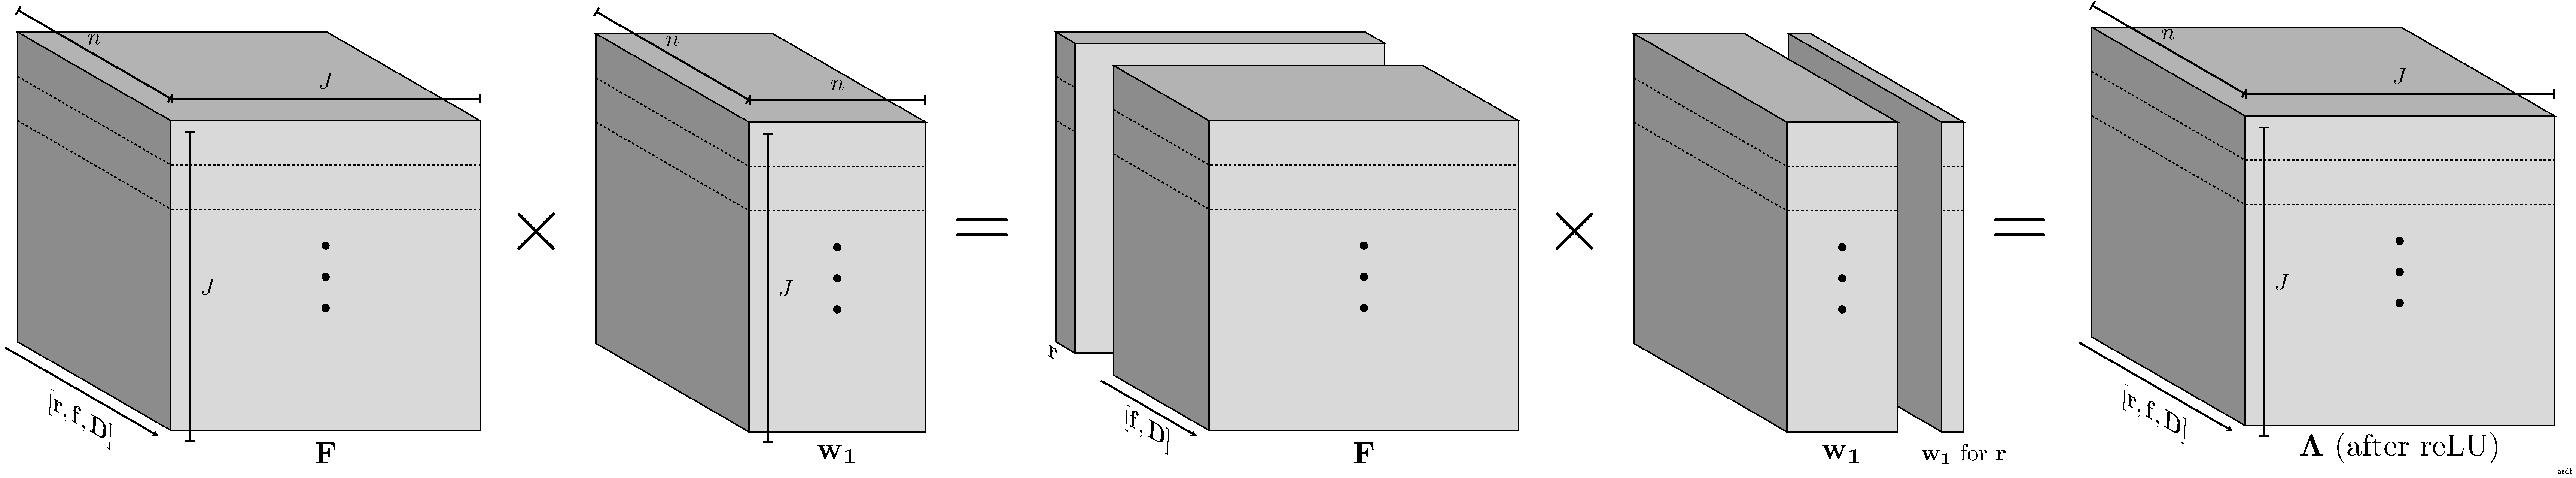
\includegraphics[width=\linewidth]{split_and_batch_multiply}
        \caption{Splitting and Batch Multiplying $\matr{F}$ and $\matr{w_1}$}
        \label{fig:Splitting and Batch Multiplying F and w1}
    \end{figure}    
    Although this preprocessing might seem applicable for the model in Identification Problem too, it does not apply fully. Since the weights $\matr{w_1}$ are updated on each iteration/epoch, we cannot multiply them with parts of $\matr{F}$ beforehand (Algorithm \ref{alg:Algorithm for the Identification Problem}). However, we can combine $\matr{D}$ and $\vect{f}$ in the preprocessing stage and simply append $\vect{r}[t]$ on each iteration, saving computation time.
    
    \subsubsection{Modeling the Linear Programming Problem in the Standard Format}
    The \texttt{scipy.optimize} module's \texttt{linprog} function requires that the arguments are in standard LP format. As discussed in \cref{sec:Calculating Rewards}, Equation \ref{eq:lp_code_constrain_rewards} resembles the standard format more closely than \ref{eq:lp_math_constrain_rewards}, but it may not be clear how so.\\
    
    Considering $\vect{u}$ and $\vect{r'}$ as variables $\vect{x}$, Equation \ref{eq:lp_code_constrain_rewards} translates into Equation \ref{eq:lp_matrix_rewards} ($J$ is the number of locations).
    \begin{equation} \label{eq:lp_matrix_rewards}
    \begin{aligned}
    & \text{minimize}
    & & \begin{bmatrix}
    \vect{0_J}\\
    \vect{1_J}\\
    \end{bmatrix}^T
    \begin{bmatrix}
    \vect{r'}\\
    \vect{u}
    \end{bmatrix}\\ \\
    & \text{subject to}
    & & \begin{bmatrix}
    I_J & -I_J\\
    -I_J & -I_J\\
    \vect{1}^T_J & \vect{0}^T_J\\
    \end{bmatrix}
    \begin{bmatrix}
    \vect{r'}\\
    \vect{u}\\
    \end{bmatrix} \leq
    \begin{bmatrix}
    \vect{r}\\
    -\vect{r}\\
    \mathcal{R}\\
    \end{bmatrix}\\
    &&& r'_i, u_i \geq 0
    \end{aligned}
    \end{equation}
    
    \section{Strange GPU Speedup in LP Computation} \label{sec:Strange GPU Speedup in LP Computation}
    Even though we intentionally transferred the rewards vector to and constrained it using \texttt{scipy.optimize} module's \texttt{linprog} function on the CPU, we obtained an unexpected GPU speedup in the LP runtimes (see \cref{sec:PriProbRes - GPU} and Figure \ref{fig:Finding Rewards - Time taken by the LP}). Confounded by this weird behavior, we wanted to pinpoint the reason(s) because SciPy's function could not have differentiated between the configurations and delivered different results. However, since this was not our research's prime motive, we did not take a strong quantitative approach in determining the cause(s).
    
    \subsection{Possible Reasons for GPU Speedup} \label{sec:Possible Reasons for GPU Speedup}
    There could have been many reasons for this bizarre behavior, including but not limited to:
    \begin{enumerate}
        \item SciPy's Optimize Module differentiating between configurations. This can be ruled out because the module could not have known the configuration during which it was called. This is because the configuration settings were applicable only on user-programmed operations, and needed to be explicitly stated - as mandated by Pytorch \cite{PTDocs}. SciPy's Optimize Module identifying the configurations is just supernatural.
        \item CPU ``set'' using exploiting more main memory than GPU ``set''. We suspected that since CPU ``set'' configuration's operations were executed solely on the CPU, the residing datasets could have used more main memory than when GPU ``set'' was running. This could have hampered the performance of LP with CPU ``set'', as the LP had lesser space to operate in. Unlike the 1\textsuperscript{st} possibility, this would have meant that CPU ``set'' was slowing down the LP, and not that GPU ``set'' was speeding up the LP.
        \item Neural network in CPU ``set'' using more CPU threads than that in GPU ``set''. The Intel i7-7700K processor is quad-core with 8 threads. Since Pytorch uses OpenMP \cite{PTDocs}, a parallel processing API for CPUs, we fancied the neural network to utilize more threads than that in GPU ``set'', thus allowing less available threads for the LP to run. 
        
        However, given that our scripts in Python did not explicitly use parallel programming with CPU ``set'' and the code was sequential, one could very well suggest that upon completion of the neural network, all threads should have been synchronized, after which the LP would have started. This would have meant that the LP's resources would have been independent of the neural network's resources, raising questions on this possibility.
    \end{enumerate}

    \subsection{LP Slowing Down or Speeding Up?} \label{sec:LP Slowing Down or Speeding Up?}
    First we determined whether the LP runtime was being sped up with GPU ``set'' or slowed down with CPU ``set''. To test this, we created a copy of our Pricing Problem's model, which focused only on logging LP runtimes at each epoch. For a baseline comparison, we scripted the same LP \textit{without} the neural network, which gave us the \underline{original} runtimes for the LP (ran for equal number of epochs), without any involvement of Pytorch modules or functions. 
    
    Comparing the former runtimes (CPU and GPU ``set'') with `Only LP' runtime (independent script) in Figure \ref{fig:LP Runtime Example for Different Configurations}, we observed that the LP in the CPU ``set'' configuration took longer to execute than that in  `Only LP' setting during each epoch. We also noticed little to no interaction between the neural network in GPU ``set'' with the LP, as the runtimes of LP in GPU ``set'' were similar to those of LP in `Only LP' setting. This confirmed that CPU ``set'' was slowing down the LP and GPU ``set'' was not speeding it up. But why?
    \begin{figure}[!htbp]
        \centering
        \begin{tikzpicture}
        \begin{axis}[
            width=\textwidth,
            height=8cm,
            xlabel=Epochs,
            ylabel=Time/s,
            scaled y ticks = false,
            grid=both,
            every axis plot/.append style={very thick},
        ]
        \addplot[red] table [col sep=comma,x=epoch, y=cpuset]{images/lp_time_logs.csv};% node [pos=0.01, scale=2, below=8pt, left=-6pt] {CPU ``set''};
        \addlegendentry{CPU ``set''}
        
        \addplot[blue] table [col sep=comma,x=epoch, y=gpuset]{images/lp_time_logs.csv};% node [pos=0.1, scale=2, above=3pt] {GPU ``set''};
        \addlegendentry{GPU ``set''}
        
        \addplot[brown] table [col sep=comma,x=epoch, y=onlylp]{images/lp_time_logs.csv};% node [pos=0.15, scale=2, above=5pt, right=5pt] {`Only LP'};
        \addlegendentry{`Only LP'}
        
        \end{axis}
        \end{tikzpicture}
        \caption[LP Runtime Example for Different Configurations]{LP Runtime Example for Different Configurations: LPs in both CPU and GPU ``set'' start running slowly, but pick up speed after $\approx$ 20 epochs. We could not explain the presence of pikes in CPU ``set'' and their absence in GPU ``set''.}
        \label{fig:LP Runtime Example for Different Configurations}
    \end{figure}
    
    
    The 2\textsuperscript{nd} hypothesis/possibility seemed more promising than the others, and we built some programs to test its various aspects, which are elaborated in next sections.
    
    \subsection{Main Memory Usage by Both Configurations}
    As the initial approach, we logged details of main memory usage when the models were running. Contrary to our expectations (again), the GPU ``set'' was utilizing more main memory than CPU ``set'' was. Precisely, when running the Pricing Problem's model with $T = 173, J = 116$ without GUI and logging at 0.2 second intervals until the model completed, the GPU ``set'' was using 9.0 - 9.1 \% of the main memory, whereas CPU ``set'' was using only 0.9 \% memory. During the tests, only 1 CPU core was utilized for GPU ``set'', whereas 6-8 cores were being used for CPU ``set''. Clearly, main memory usage wouldn't have been the reason for the strange GPU speedup in LP runtime as LP's GPU ``set'' runtime would have been lower if the relation with main memory usage was true. However, there could be a relation between CPU usage and LP runtime.
    
    \begin{figure}[!htbp]
        \centering
        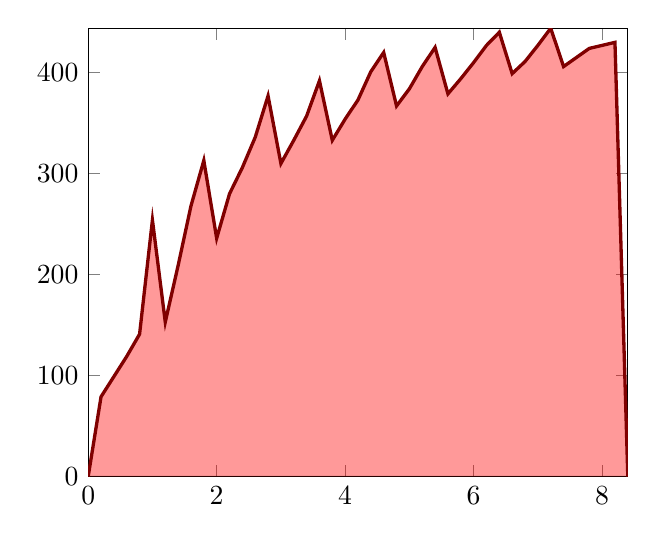
\begin{tikzpicture}
        \begin{axis}[
        domain=0:10,
        enlargelimits=false,
        ]
        %
        \addplot[fill=red, opacity=.4, domain=0:10] coordinates {
            (0.0, 0)
            (0.2, 79.0)
            (0.4, 99.0)
            (0.6, 119)
            (0.8, 141)
            (1.0, 254)
            (1.2, 153)
            (1.4, 209)
            (1.6, 268)
            (1.8, 313)
            (2.0, 236)
            (2.2, 280)
            (2.4, 306)
            (2.6, 336)
            (2.8, 377)
            (3.0, 310)
            (3.2, 333)
            (3.4, 357)
            (3.6, 392)
            (3.8, 333)
            (4.0, 354)
            (4.2, 373)
            (4.4, 401)
            (4.6, 420)
            (4.8, 367)
            (5.0, 384)
            (5.2, 406)
            (5.4, 425)
            (5.6, 379)
            (5.8, 394)
            (6.0, 410)
            (6.2, 427)
            (6.4, 440)
            (6.6, 399)
            (6.8, 411)
            (7.0, 427)
            (7.2, 444)
            (7.4, 406)
            (7.6, 415)
            (7.8, 424)
            (8.0, 427)
            (8.2, 430)
            (8.4, 0)
        }\closedcycle;
        
        \addplot [very thick, red!50!black] coordinates {
            (0.0, 0)
            (0.2, 79.0)
            (0.4, 99.0)
            (0.6, 119)
            (0.8, 141)
            (1.0, 254)
            (1.2, 153)
            (1.4, 209)
            (1.6, 268)
            (1.8, 313)
            (2.0, 236)
            (2.2, 280)
            (2.4, 306)
            (2.6, 336)
            (2.8, 377)
            (3.0, 310)
            (3.2, 333)
            (3.4, 357)
            (3.6, 392)
            (3.8, 333)
            (4.0, 354)
            (4.2, 373)
            (4.4, 401)
            (4.6, 420)
            (4.8, 367)
            (5.0, 384)
            (5.2, 406)
            (5.4, 425)
            (5.6, 379)
            (5.8, 394)
            (6.0, 410)
            (6.2, 427)
            (6.4, 440)
            (6.6, 399)
            (6.8, 411)
            (7.0, 427)
            (7.2, 444)
            (7.4, 406)
            (7.6, 415)
            (7.8, 424)
            (8.0, 427)
            (8.2, 430)
            (8.4, 0)
        };
        \end{axis}
        \end{tikzpicture}
    \end{figure}
    
    \subsubsection{asdf}
\end{appendices}